% Point 4 manuscript fragment (not a standalone LaTeX file).
% Required in the parent preamble: \usepackage{graphicx,amsmath,booktabs}
% Place the four PNG files from figures/ into your project's figs/ directory.
\subsection{Semantic Non-Alignment and Emergent Discussion Themes}\label{sec:point4}

\paragraph{Methodology.}
We examined 195 linked Telegram channel--discussion-group pairs (98 crypto and 97 conspiracy), with 134,984 observed channel posts and 513,973 sampled group messages (up to 5,000 per pair under the existing sampling protocol). After excluding 40,411 messages shorter than five characters, we embedded 473,562 messages with \texttt{OpenVINO/Qwen3-Embedding-0.6B-int8-ov}. Further excluding URL-only, mention-only and other non-lexical messages yielded 445,584 semantically eligible group messages. For each message $g$ in group $i$, we calculated the maximum cosine similarity to the linked channel corpus $C_i$:
\begin{equation}
  s(g,C_i)=\max_{c\in C_i}\cos\bigl(E_q(g),E_d(c)\bigr).
\end{equation}
A message was operationally \emph{non-aligned} (\emph{group-only}) if $s(g,C_i)<0.52$. The cutoff was chosen before the full run using a balanced 100-item calibration exercise, and 0.50 and 0.55 were retained for sensitivity checks. The primary comparison was the unweighted average of pair-level non-alignment rates; pair-level bootstrap intervals and a Welch test were used for inference.

\paragraph{Non-alignment rates.}
At the prespecified cutoff, 334,080 eligible group messages were operationally non-aligned (169,406 crypto and 164,674 conspiracy). The equal-pair mean rates were \textbf{74.68\%} (95\% bootstrap CI 71.68--77.57\%) in crypto and \textbf{76.11\%} (71.48--80.50\%) in conspiracy (Table~\ref{tab:p4-rates}). Their difference (conspiracy minus crypto) was $+1.43$ percentage points (95\% CI $-3.95$ to $+6.74$; Welch $p=0.606$). We thus found no convincing evidence of a difference in mean rates; this is not a test of equivalence. Between-pair dispersion was higher in conspiracy (SD 22.91 vs. 14.84 percentage points; exploratory Brown--Forsythe $p=0.0058$).

\begin{table}[t]
\centering
\caption{Operational semantic non-alignment at cosine-similarity threshold 0.52. The principal estimator weights channel--group pairs equally.}
\label{tab:p4-rates}
\begin{tabular}{lrr}
\toprule
Measure & Crypto & Conspiracy\\
\midrule
Pairs & 98 & 97\\
Semantically eligible messages & 226,100 & 219,484\\
Operationally non-aligned messages & 169,406 & 164,674\\
Mean pair-level rate & 74.68\% & 76.11\%\\
95\% bootstrap CI & 71.68--77.57\% & 71.48--80.50\%\\
Median pair-level rate & 77.16\% & 84.28\%\\
Between-pair SD (percentage points) & 14.84 & 22.91\\
\bottomrule
\end{tabular}
\end{table}

\begin{figure}[t]
\centering
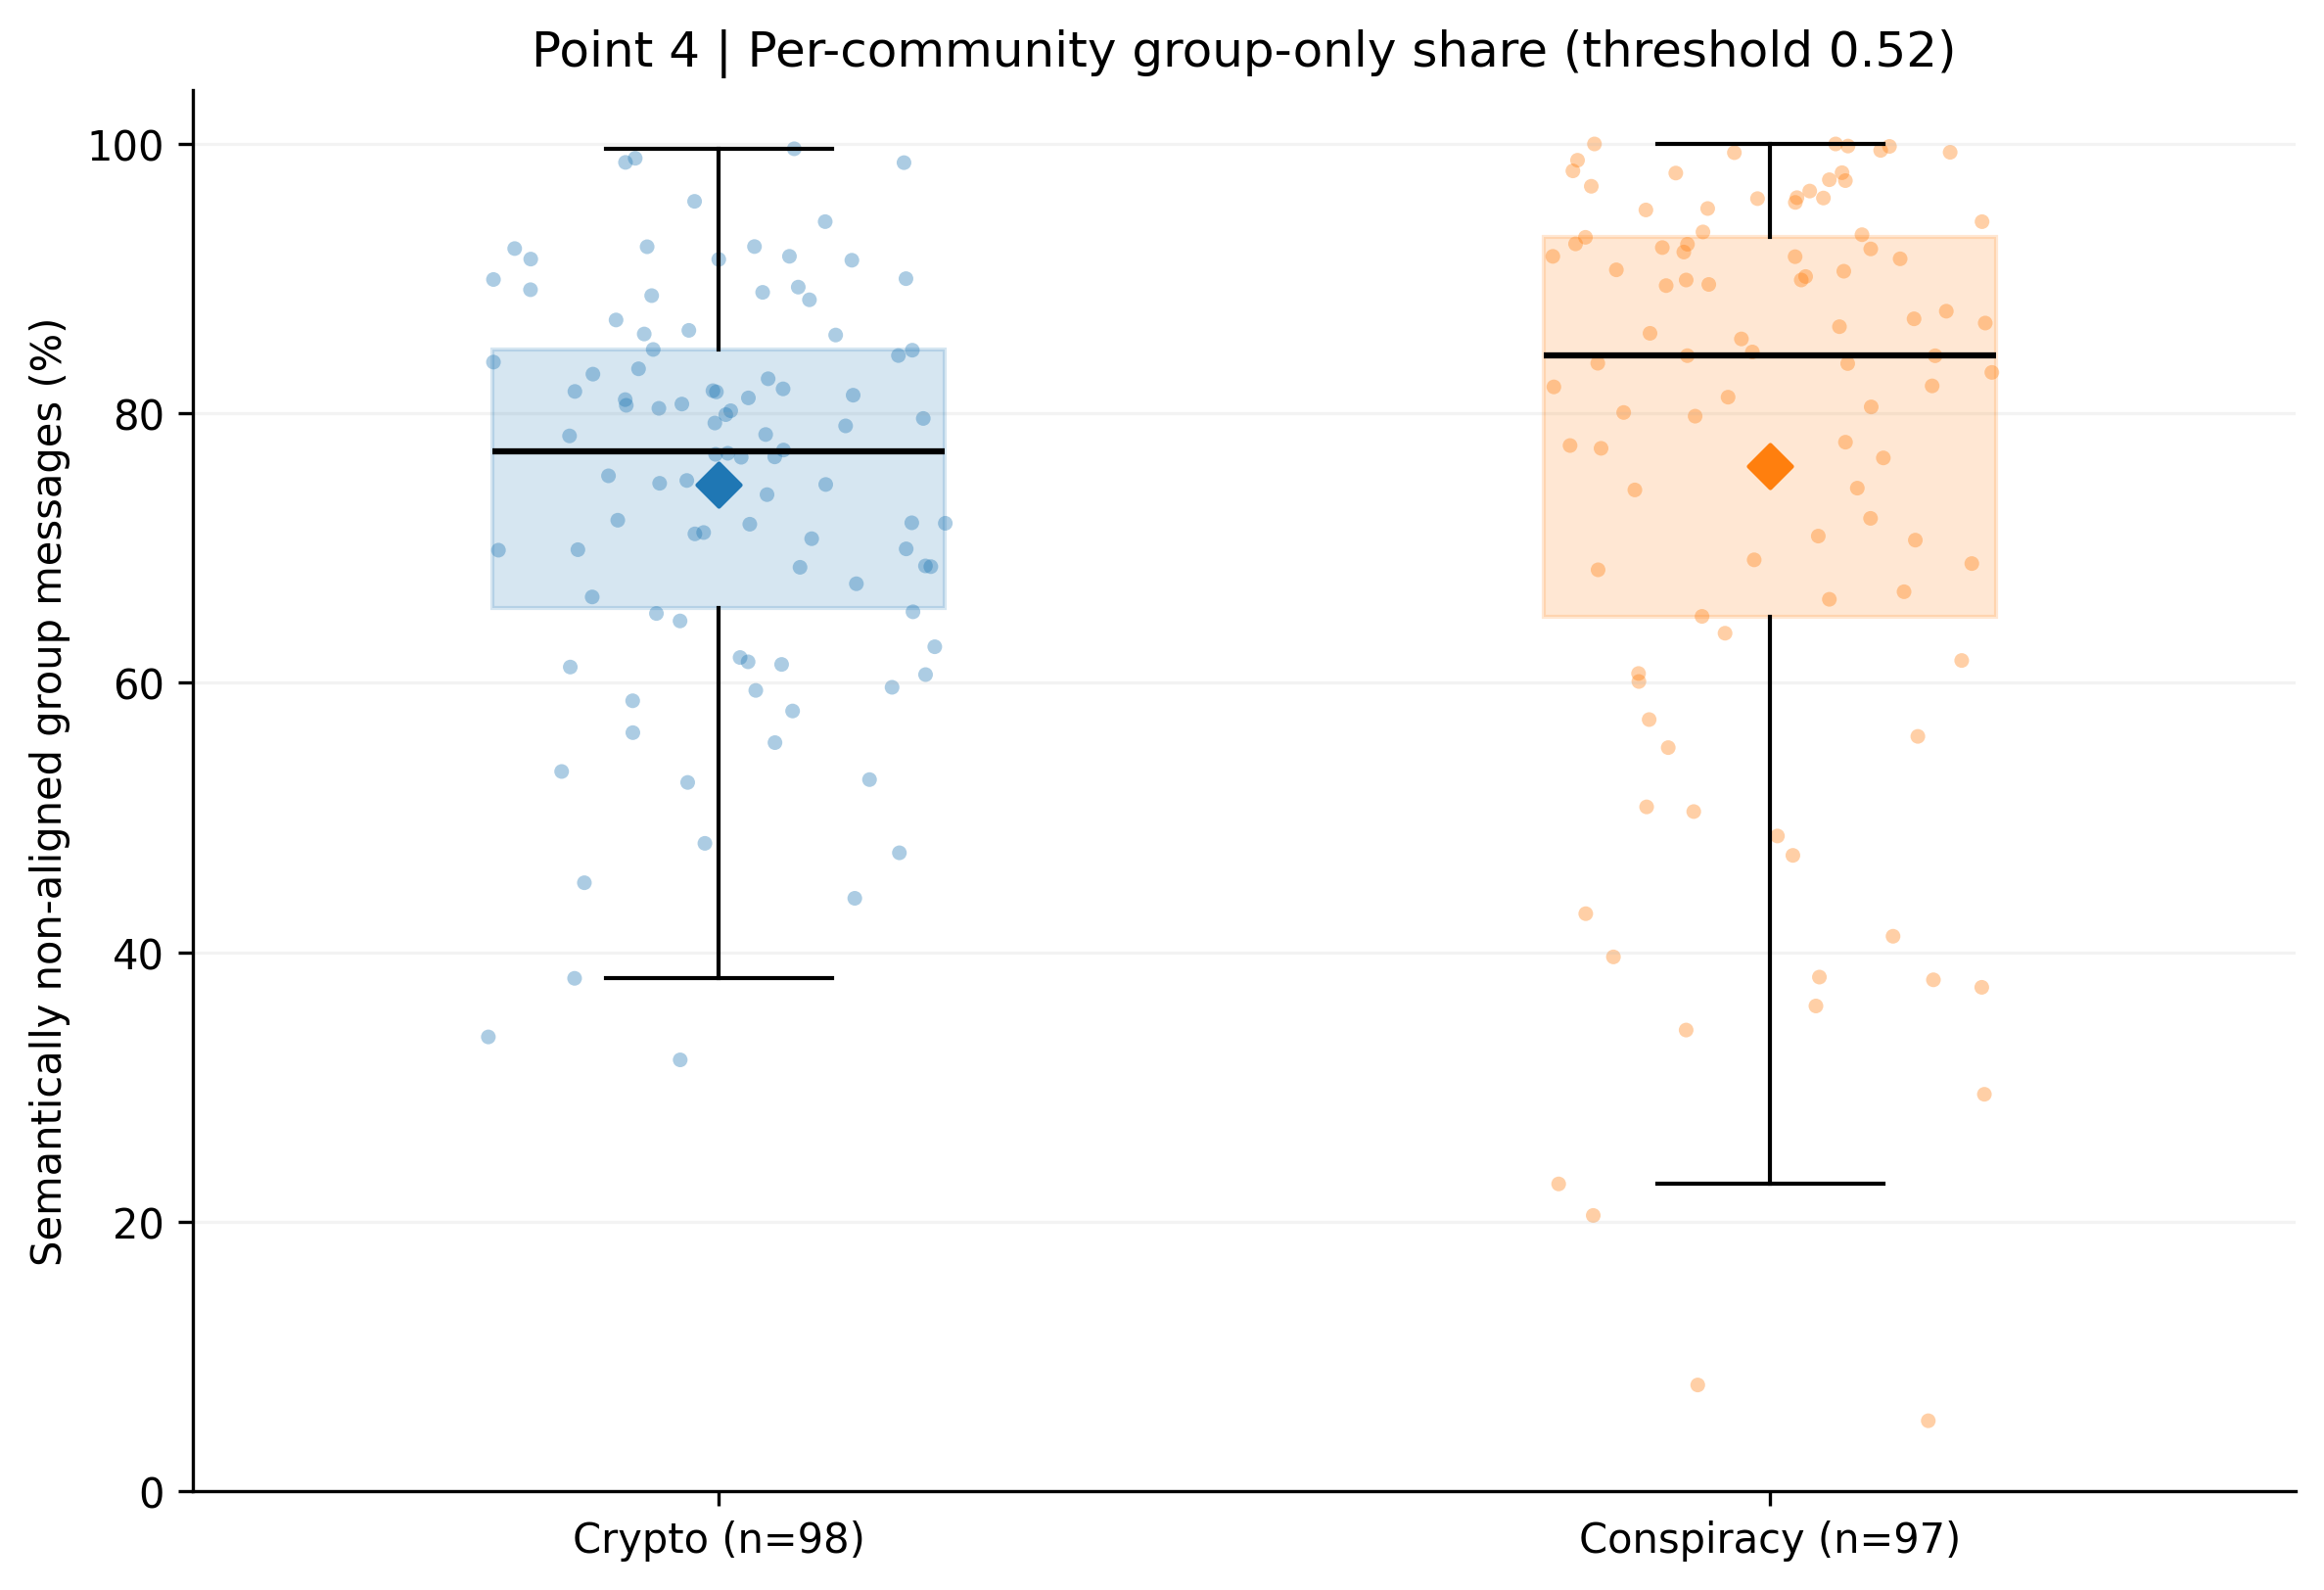
\includegraphics[width=\linewidth]{figs/figure_1_pairwise_rates.png}
\caption{Distribution of per-pair semantic non-alignment rates. Points represent channel--group pairs; diamonds represent equal-pair category means.}
\label{fig:p4-rates}
\end{figure}

\paragraph{Reference-corpus effects and robustness.}
The median number of distinct channel posts was 83 in crypto versus 237 in conspiracy. Non-alignment decreased as the number of candidate channel posts increased (Spearman's $\rho=-0.420$ in crypto and $-0.827$ in conspiracy; both $p<0.001$; Figure~\ref{fig:p4-channel-size}). This is partly structural: a maximum-over-candidates similarity score cannot decrease when more candidates are added for a fixed query. At thresholds 0.50, 0.52 and 0.55, equal-pair non-alignment rates were 69.42\%, 74.68\% and 80.56\% in crypto, compared with 69.94\%, 76.11\% and 83.37\% in conspiracy (Figure~\ref{fig:p4-threshold}). Weighting normalized texts once or capping repeated-text frequency at five had only modest effects on category means but could noticeably change individual pairs.

\begin{figure}[t]
\centering
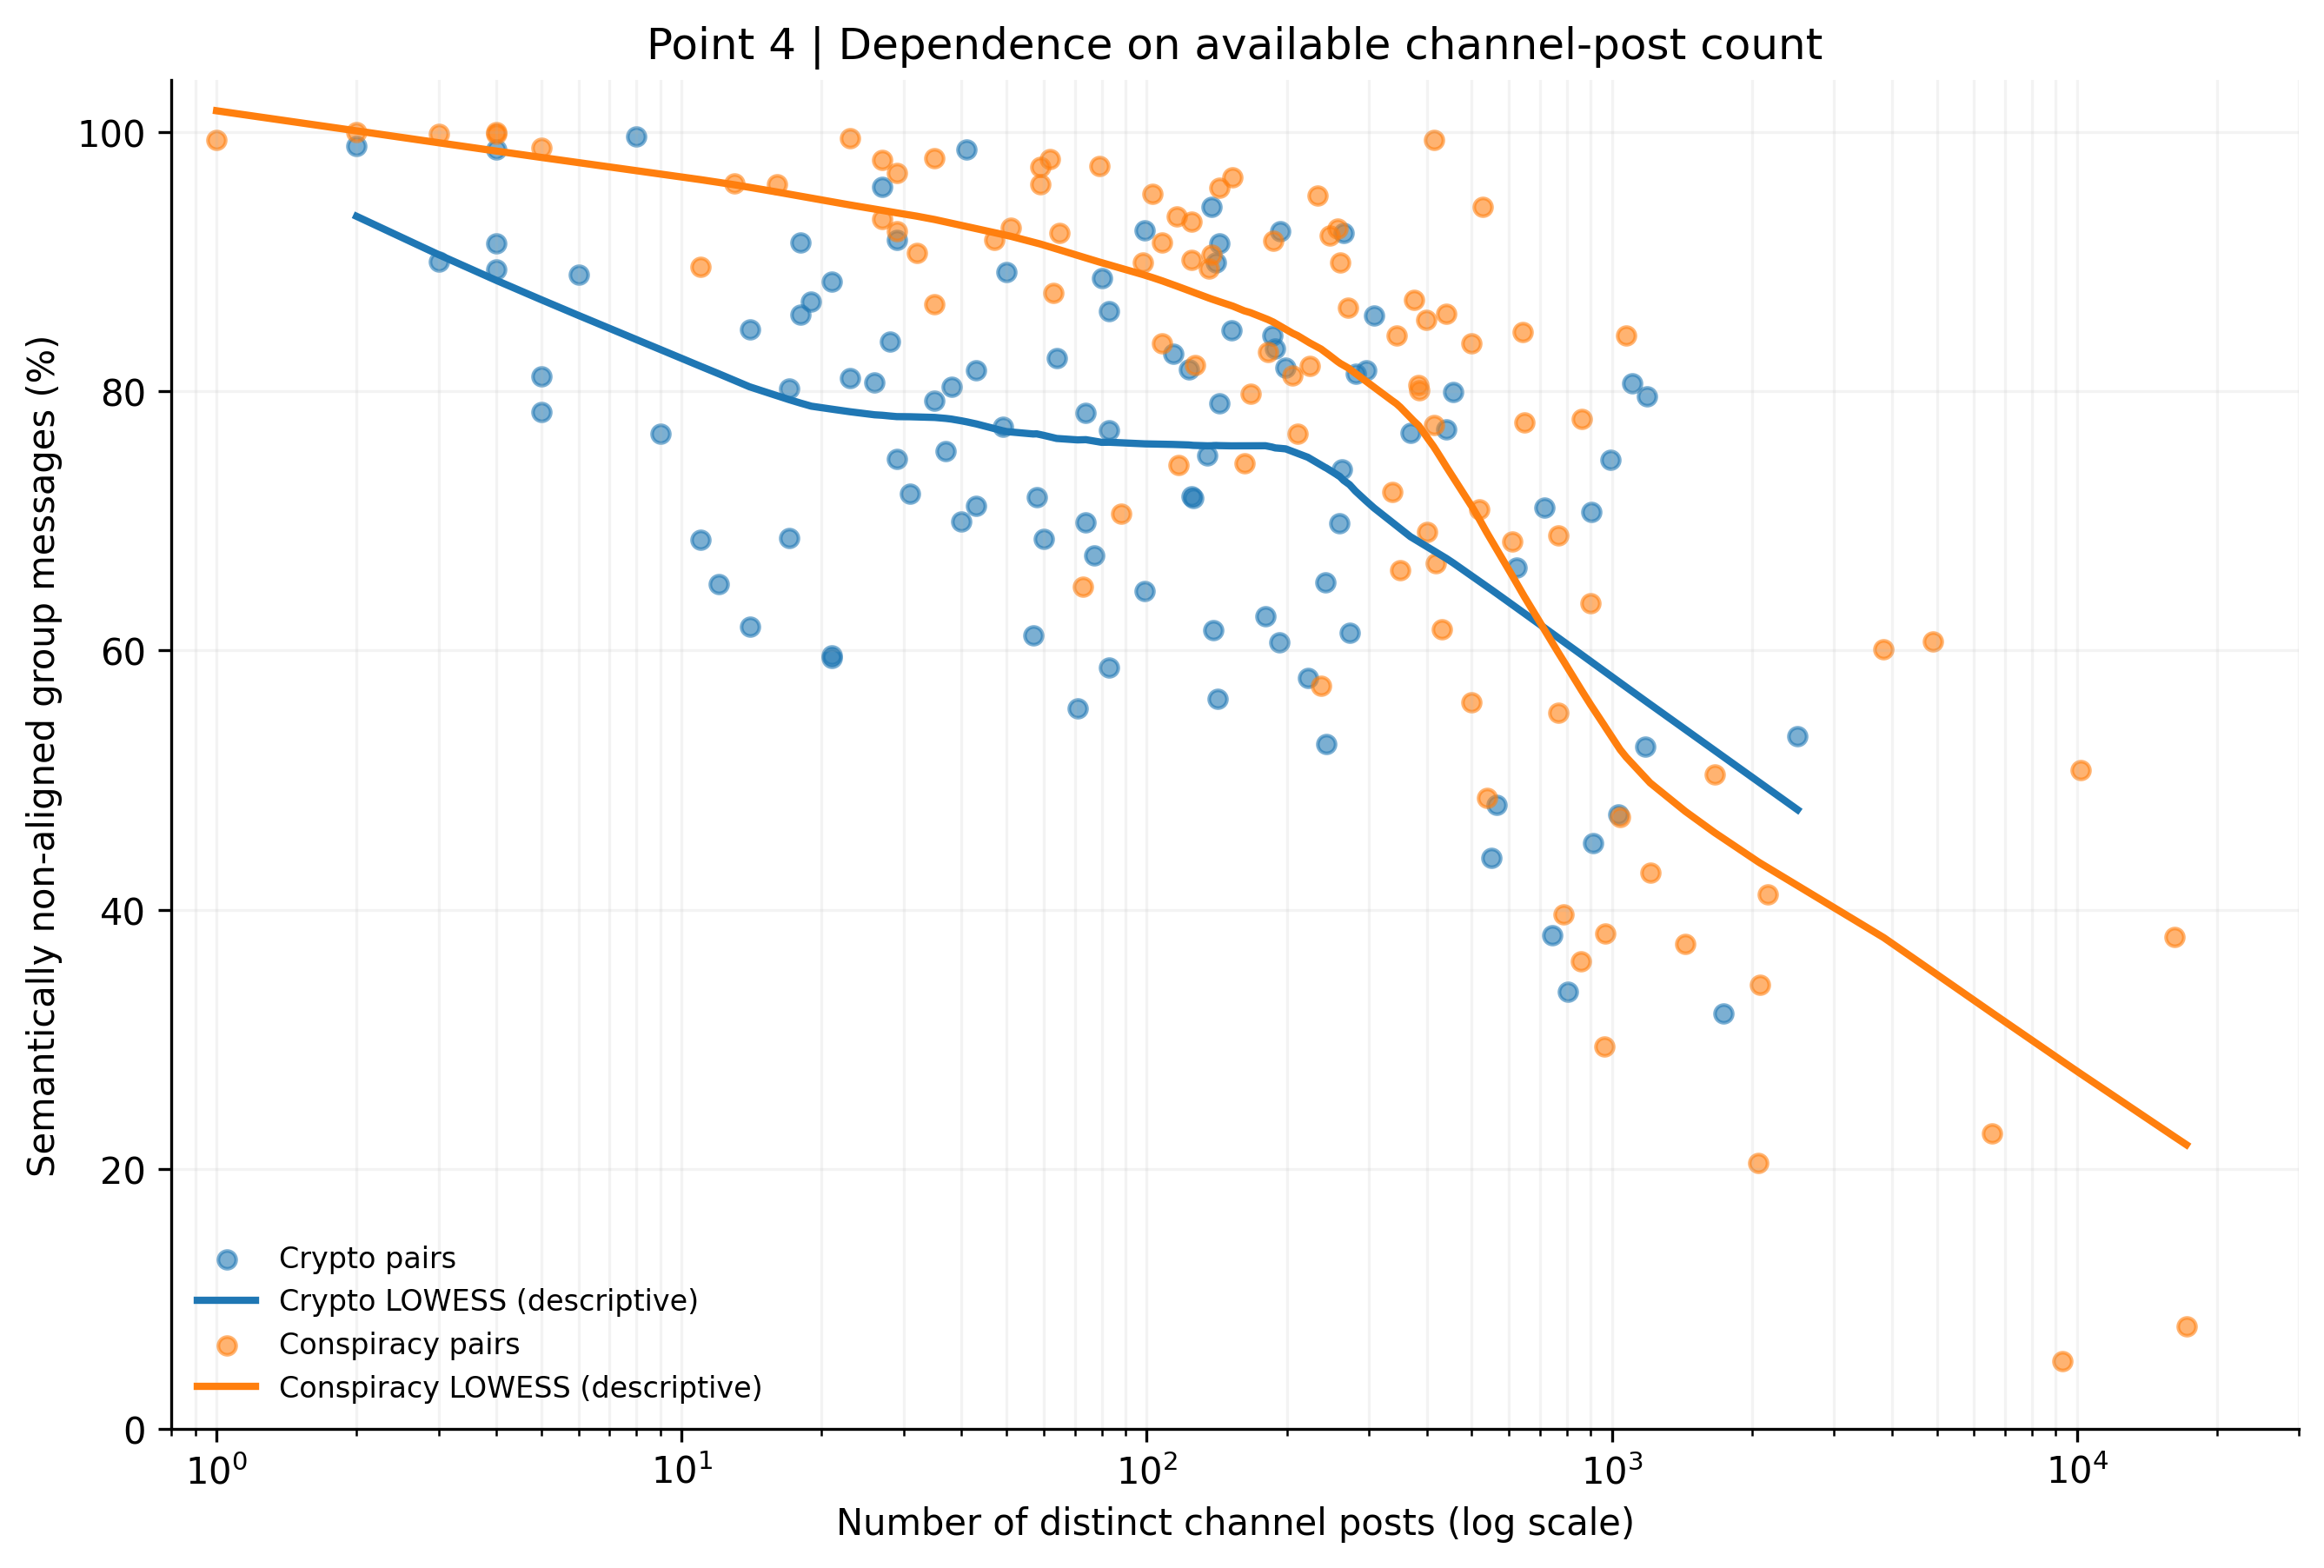
\includegraphics[width=\linewidth]{figs/figure_2_channel_corpus_size.png}
\caption{Association between channel reference-corpus size and operational non-alignment rate.}
\label{fig:p4-channel-size}
\end{figure}

\begin{figure}[t]
\centering
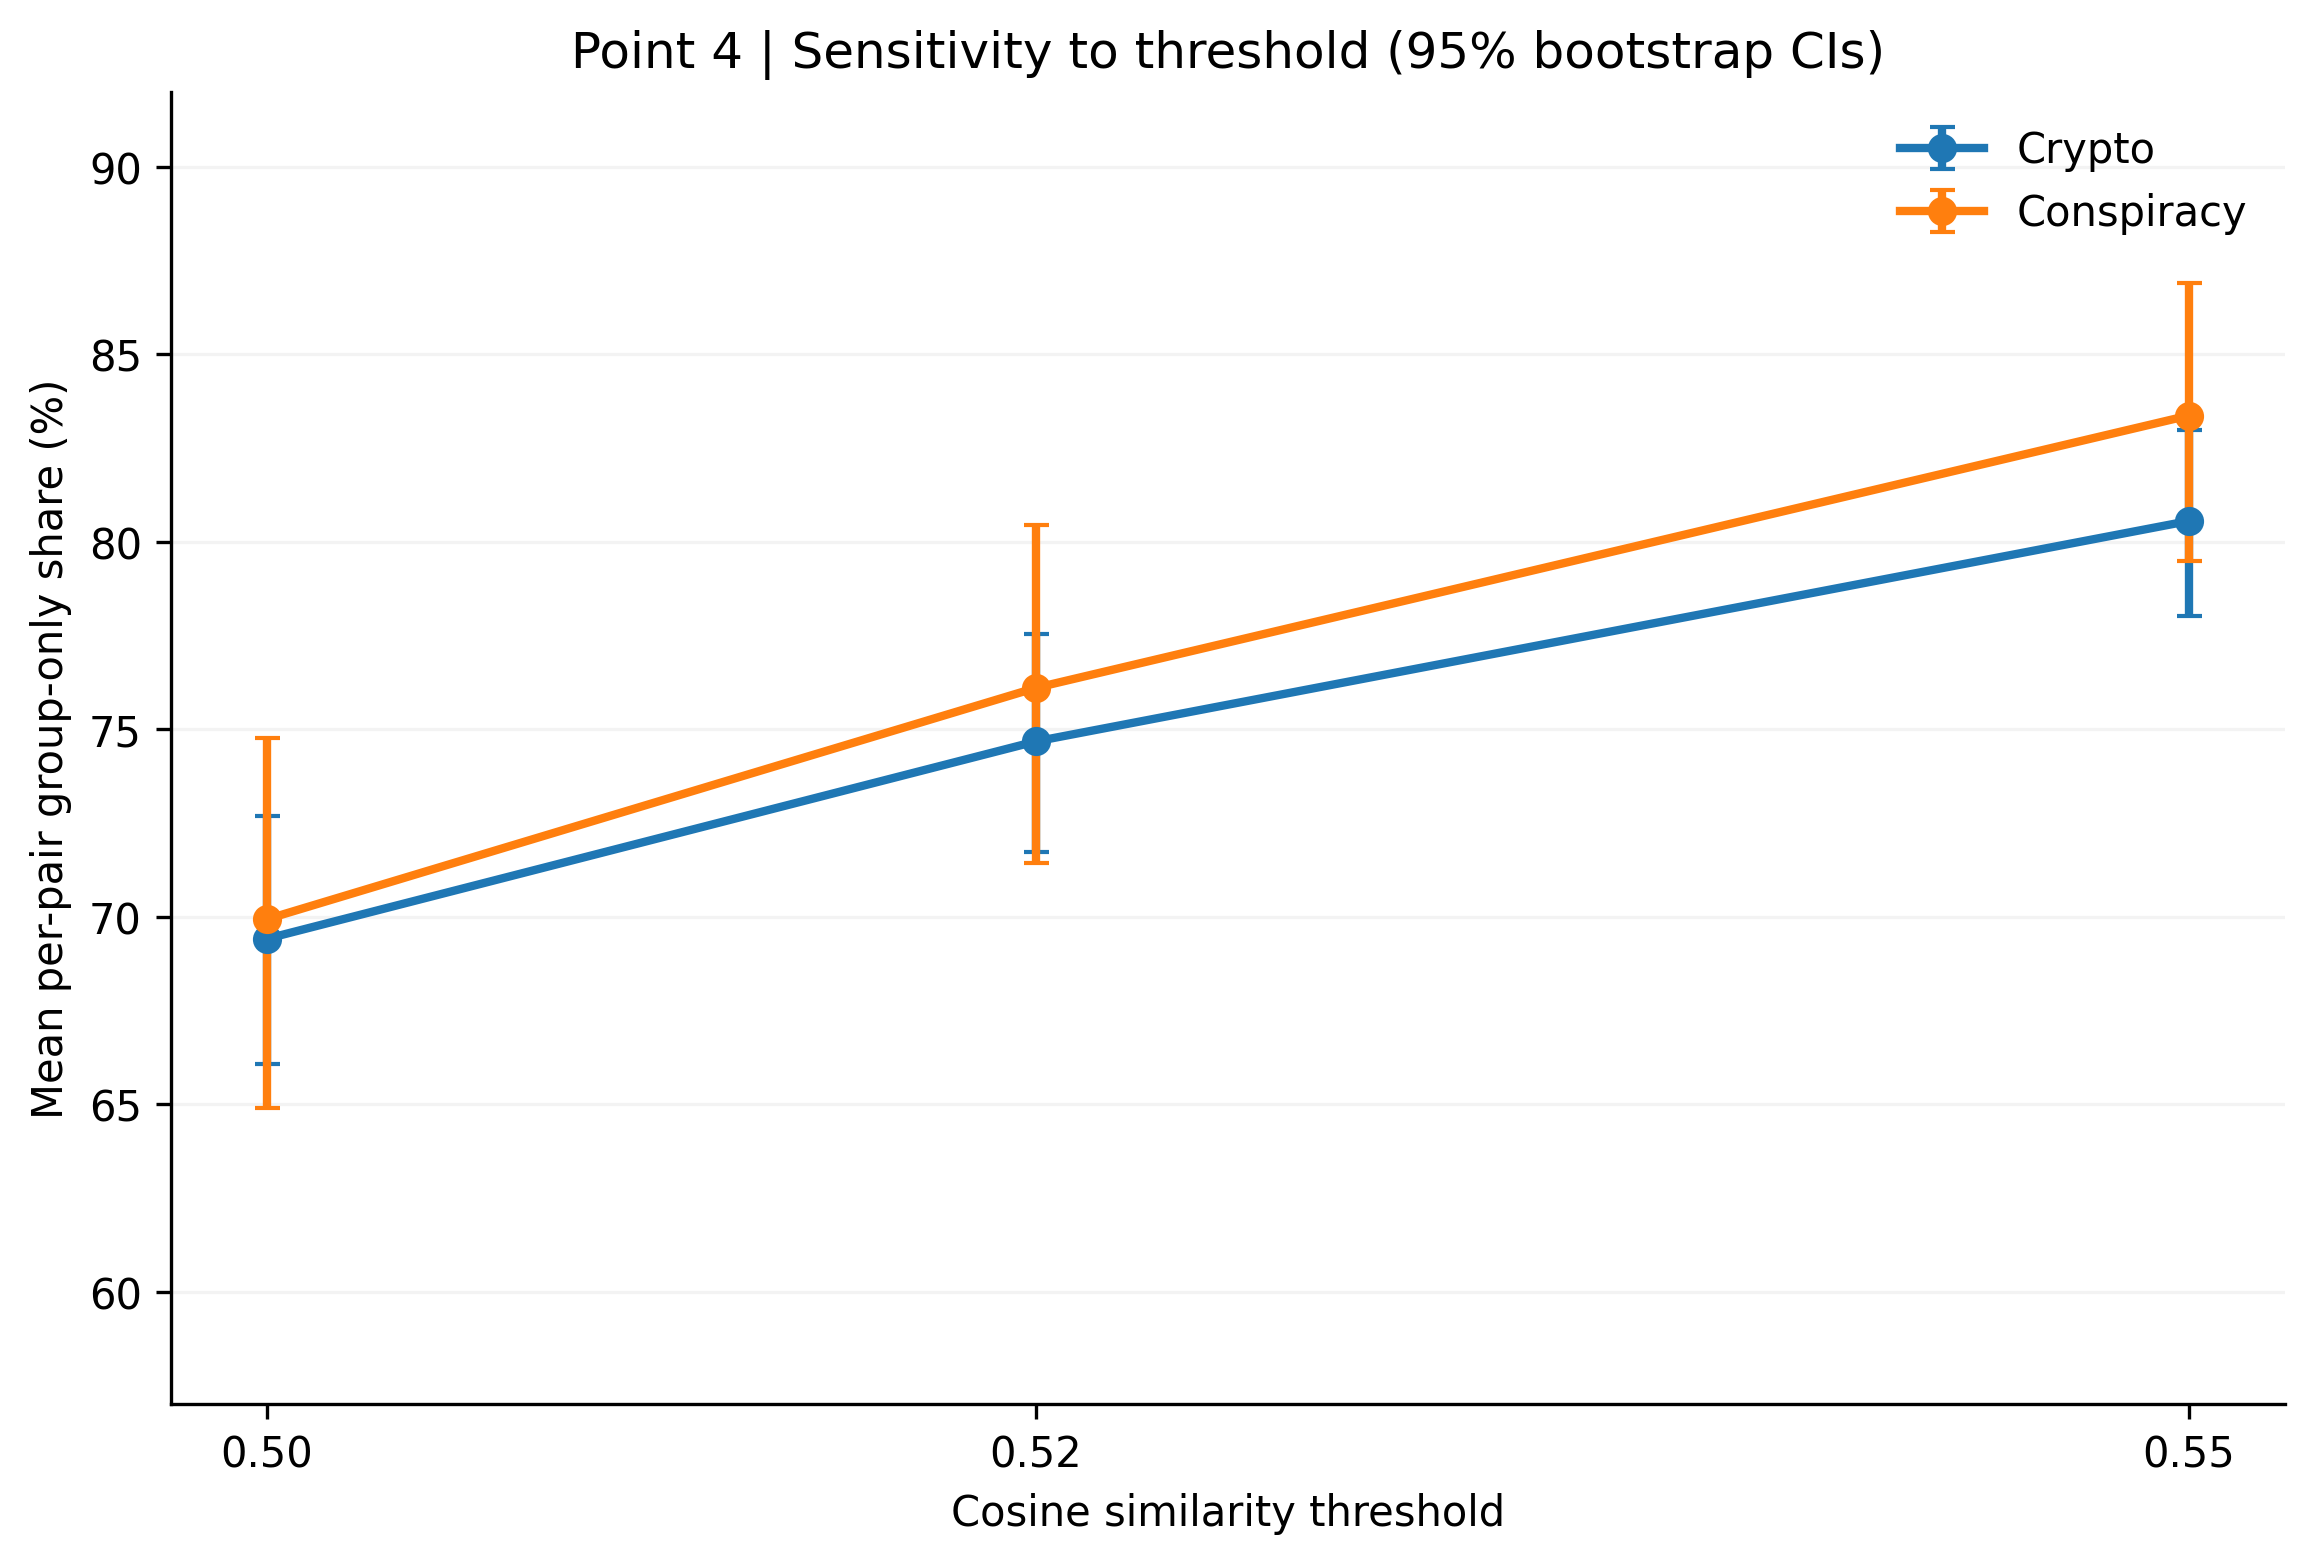
\includegraphics[width=\linewidth]{figs/figure_3_threshold_sensitivity.png}
\caption{Threshold sensitivity of the equal-pair mean non-alignment rate; 0.52 is the primary cutoff.}
\label{fig:p4-threshold}
\end{figure}

\paragraph{Exploratory content characterization.}
Embedding-based clustering of 284,068 distinct within-pair non-aligned texts was used only to discover candidate topics, not to estimate their prevalence. A separate, reproducible sample of six non-aligned message instances per pair (1,170 messages: 588 crypto, 582 conspiracy) was then coded along two axes, communicative function and primary subject, with interpretability and promotion flags. This was a single-pass, text-only, rule-guided exploratory procedure with targeted case review; no independent reference-label validation or inter-rater reliability measure is available. Five thousand pair/within-pair bootstrap draws provide sampling intervals conditional on assigned labels, not correction for coding error.

The assigned \emph{greeting/social interaction} label occurred on 20.9\% of crypto versus 4.3\% of conspiracy messages (difference $-16.6$ percentage points, 95\% interval $-22.4$ to $-11.0$). \emph{Information/news sharing} occurred on 2.6\% versus 22.3\% (difference $+19.8$ points; interval $+14.1$ to $+26.0$); \emph{substantive discussion/opinion} occurred on 25.9\% versus 32.0\% (difference $+6.1$ points; interval $-1.6$ to $+14.0$). These are descriptive contrasts in assigned codes, not validated thematic prevalence (Figure~\ref{fig:p4-functions}). The proportion of messages without an identifiable specific subject was high: \emph{No clear theme} was assigned to 60.2\% in crypto and 34.9\% in conspiracy, while \emph{Unclear} accounted for 16.8\% and 12.9\%. Identifiable subject cues included markets, rewards, technical support, politics, health, religion and geopolitics.

\begin{table}[t]
\centering
\caption{Exploratory pair-equal communicative-function shares among sampled operationally non-aligned messages. Intervals reflect sampling variability conditional on labels, not coding accuracy.}
\label{tab:p4-functions}
\small
\begin{tabular}{lrr}
\toprule
Assigned function & Crypto & Conspiracy\\
\midrule
Greeting/social interaction & 20.9\% & 4.3\%\\
Question or help request & 15.0\% & 14.8\%\\
Substantive discussion/opinion & 25.9\% & 32.0\%\\
Information/news sharing & 2.6\% & 22.3\%\\
Promotion/solicitation & 5.3\% & 9.1\%\\
Moderation/security & 1.7\% & 0.7\%\\
Other/unclear & 28.7\% & 16.8\%\\
\bottomrule
\end{tabular}
\end{table}

\begin{figure}[t]
\centering
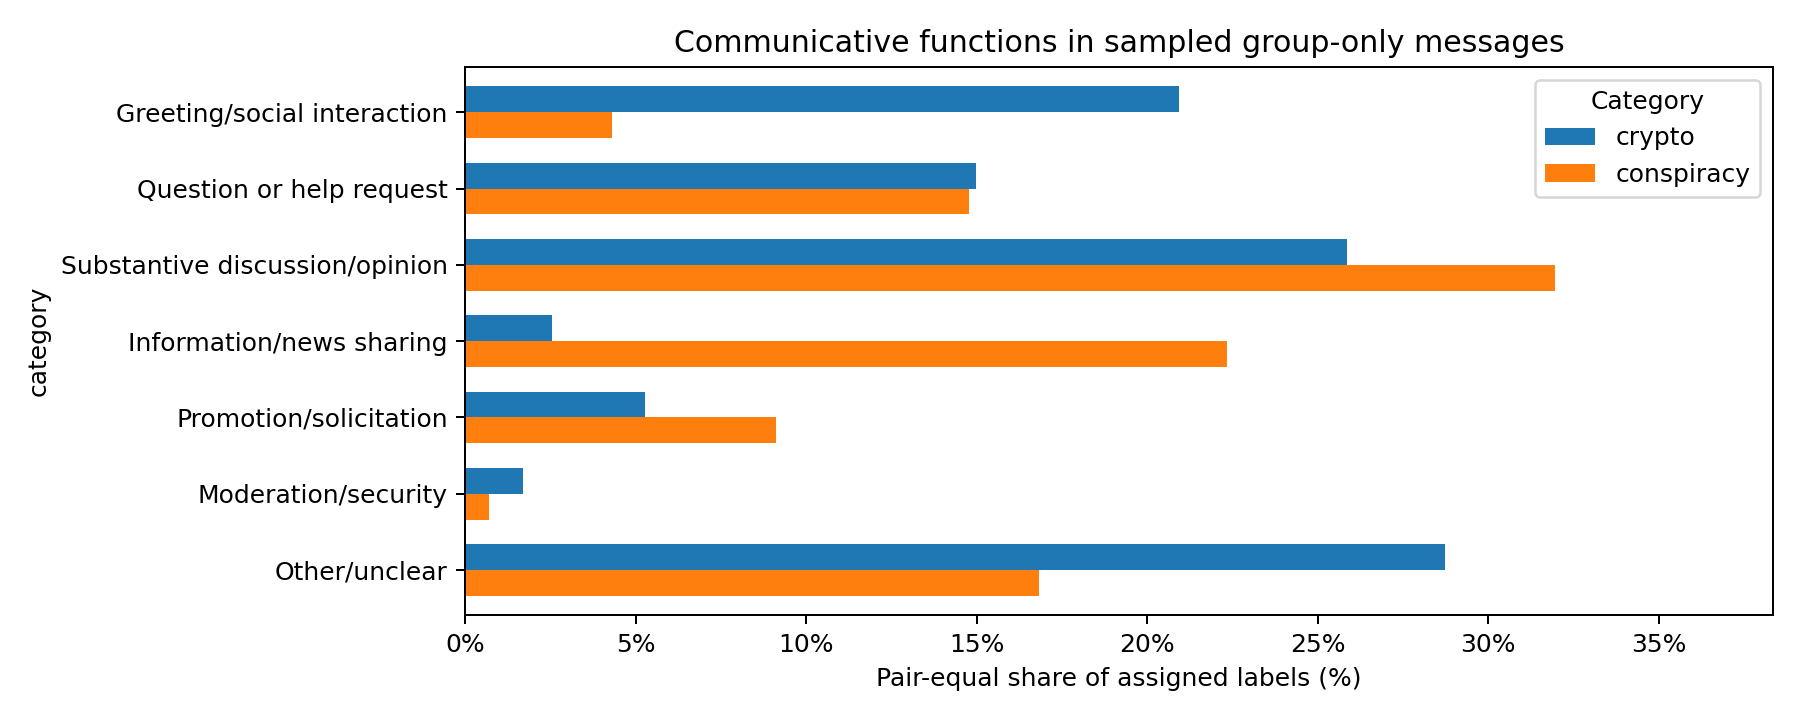
\includegraphics[width=\linewidth]{figs/figure_4_communicative_functions.png}
\caption{Exploratory pair-equal shares of assigned communicative-function labels among 1,170 sampled operationally non-aligned messages. These coding proportions lack independent label validation.}
\label{fig:p4-functions}
\end{figure}

\paragraph{Interpretation and limitations.}
These results measure semantic non-alignment with the \emph{observed} channel corpus, not causal independence or the origin of a discussion. In particular, the reference corpus was not restricted to posts predating each group message. Unequal channel-post counts, retrieval-model behavior, similarity cutoff, message-sampling limits, duplicate content, multilingualism and short/context-poor messages all affect interpretation. Median length in the thematic sample was 26 characters in crypto versus 92.5 in conspiracy; 66.3\% versus 29.4\% were under 40 characters. The thematic sample received no independent coding-accuracy evaluation, so its percentages must remain exploratory. The strongest supported finding is the prevalence and heterogeneity of operational \emph{semantic non-alignment}, with the thematic labels offering preliminary context rather than proof of new or autonomous community topics.
